\chapter{Introduction}\label{C:intro}

\subsection{The reinforcement learning problem}

Reinforcement learning is a framework that describes how an agent learns by interacting with the environment. The framework involves 2 entities the agent and environment. The agent is the only entity that we as designers have direct control of. We decide how its learns and decides on its actions. The environment is the context and situation that the agent is in. There are three important flows of information;  the state of the environment to the agent, the action decision to the environment and lastly the reward to the agent. This can be best be understood in the figure below.

\begin{fig}
\begin{center}
    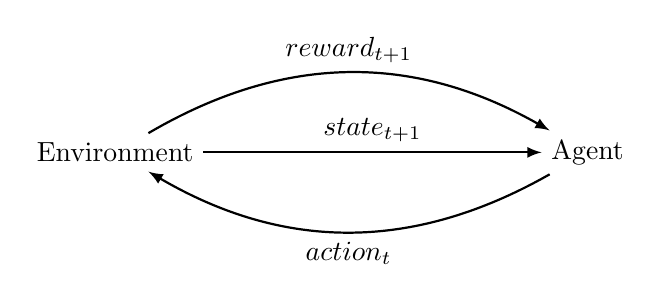
\begin{tikzpicture}[
        node distance=6cm, % Increased node distance for better spacing
    ]
        % Define nodes
        \node (env) {Environment};
        \node (agent) [right of=env] {Agent};

        % Define arrows and labels without boxes
        \draw [-latex,bend left, thick] (env) edge node[anchor=south] {$reward_{t+1}$} (agent);
        \draw [-latex, thick] (env) -- node[anchor=south] {$state_{t+1}$} (agent);
        \draw [-latex,bend left,thick] (agent) edge node[anchor=north] {$action_{t}$} (env);
    \end{tikzpicture}
    \caption{The flow of information between th environment and agent}
\end{center}
\end{fig}

The state is a representation of the information within the environment that the agent observes to make its decision on which action to take. The reward signal is treated as the final word on how good the previous state action was, the more reward the better, always. Lastly the action taken by the agent is sent to the environment and the environment will in turn return the next state and reward. This brings us to the reinforcement learning problem which can be framed as such "How does the agent decide which actions to take given the state such that it maximises the future cumulative reward". It is important that the agent maximises all \textit{future cumulative} reward otherwise short term gains could be made to the sacrifice of larger long term gains. This idea has been formalised by Richard Sutton as the reward hypothesis

\begin{quote}
    "That all of what we mean by goals and purposes can be well thought of as maximization of the expected value of the cumulative sum of a received scalar signal (reward)." 
    \cite{suttonReinforcementLearningSecond2018}
    \label{quote:reward}
\end{quote}

\subsection{Formalism}

The reinforcement problem can be formalised as a Markov Decision Process (MDP). The MDP is a collection of states, actions and rewards along with a transition function which states the probability of the next reward and state given a state and reward. This makes the MDP a 4-tuple $(S,\mathcal{A}, \mathcal{P}, R)$ where $S$ is the set of states, $\mathcal{A}(s)$ is the set of actions that can be taken from state $s$, $\mathcal{P}$ is the transition function and $R \subset \mathbb{R}$ is the set of rewards. The transition function is defined as:

\begin{equation}
\mathcal{P}(s',r, s,a) = Pr\left\{ S_{t}=s', R_{t}=r | S_{t-1}=s, A_{t-1}=a \right\}
\label{eq:transition}
\end{equation}
Where $s,s \in S, a \in \mathcal{A}(s) \text{ and } r \in R$.

This transition function completely characterises the dynamics of the environment. The abstraction of the environment to a MDP is widely applicable and serves as the basis for much of reinforcement learning. We can see here that transition function only looks at the previous state. It can do this because we assume that the state representation has the \textit{Markov property} \cite{suttonReinforcementLearningSecond2018}. The Markov property states that including previous states in the conditional wont change the probability of next state reward tuple. In other words $\mathcal{P}(s_{t+1}, r_{t+1}, s_{t},a_{t}) = \mathcal{P}(s_{t+1}, r_{t+1}, s_{t},a_{t}, s_{t-1}, s_{t-2}, ... , s_{0})$. Therefore a state with the Markov property is a sufficient representation of the history of the agent-environment interaction. In some problems the agent only partially observes the state meaning the Markov property is not satisfied. This is called a partially observable MDP (POMDP) and is a more complex problem to solve which wont be addressed in this report.

The agent interacts with the MDP to produce a trajectory of states, actions and rewards. Because the agent will not know the transition function \ref{eq:transition} it will have to learn about the MDP from the information in a trajectory \ref{eq:MDPsequence}.

\begin{equation}
S_{1},A_{1},R_{2},\dots S_{n},A_{n}, R_{n+1},\dots 
\label{eq:MDPsequence}
\end{equation}

In this trajectory \ref{eq:MDPsequence} we have an infinite sequence as this is an example from a continuing MDP that has no end. Alternatively you could have episodic MDPs that have a start and end with a terminal state. Episodic MDPs require practical considerations in implementing algorithms. However for most of the theory it make no difference as you can think of a episode MDP as a continuing MPD with a state that transitions to itself and gives reward 0.

"The cumulative sum of a received scalar signal" part of the reward hypothesis \ref{quote:reward} can be formalised to be the return $G$.

\begin{equation}
G_{t}=R_{t+1}+\gamma R_{t+2}+\gamma^{2}R_{t+3}\dots=\sum_{k=t}^{\infty}\gamma^{t-1}R_{t+1}
\end{equation}

$\gamma$ is called the discounting factor and weights future rewards to have less effect on the return. It is usually added for two reasons. Firstly because it makes the return finite which simplifies the mathematics. Secondly is due to the very natural intuition that the future is less predicable than the present, thus more distance rewards should have less weight as they are less certain. 


A agent will use policy $\pi$ which provides the probability of taking action $a$ given state $s$. This policy could be deterministic or stochastic.
To evaluate how good a policy is or how much reward we can expect at a state we need a function to tell us. This is called the value function and it is a expectation of the future rewards.

\begin{equation}
v_{\pi}(s)=\mathbb{E}\left[ G_{t}| S_{t}=s\right] 
\end{equation}

The state value function depends on the state, policy and discounting factor $\gamma$ which is used by the return. In a similar vain to the state value function we have the action-value function which is the expected future reward given a state and action taken.

\begin{equation}
q_{\pi}(s,a) = \mathbb{E}\left[ G_{t} | S_{t}=s, A_{t}=a \right] 
\end{equation}

We can understand how to compute the expectation of the value function by looking at the Bellman equation \cite{suttonReinforcementLearningSecond2018}. The Bellman equation is based off the notion that the value of a situation should be the immediate reward you get plus the value of the situation you end up in. This can be written for the state value function as follows:

\begin{equation}
v_{\pi}(s)=\sum_{a}\pi(a|s)\sum_{s',r}p(s',r|s,a)\left[ r+\gamma v_{\pi}(s') \right]
\end{equation}
$\pi(a|s)$ is the probability of taking action $a$ given state $s$ and $p(s',r|s,a)$ is the transition function. This equation can be solved for $v_{\pi}$ by iterating over all states and actions until the value function converges. This is called the iterative policy evaluation and is a dynamic programming technique \cite{bellmanDynamicProgramming1957}.

The maximising part of the reinforcement problem can be solved by the finding optimal actions. We can define both $v_{\star}=\underset{ \pi }{ \text{max} }\ v_{\pi}(s)$ and $q_{\star}=\underset{ \pi }{ \text{max} }\ q_{\pi}(s,a)$ as the optimal value given optimal actions afterwards.
If we can find $q_{\star}$ then the problem is solved as we could make a policy $\pi_{\star}$ that is greedy with respect to $q_{\star}$. Two things stop this from being so simple. Firstly is that in many real problems we don't know the true transition function, therefore we either have to learn/approximate or learn the value/policies in a way that doesn't involve the transition function. Secondly is the computational complexity of iterating over all states and actions as well as all possible policies. This is called the curse of dimensionality and is a major problem in reinforcement learning. If we try to learn and transition funtion and come up with a model of the environment then we are using model based methods, alternatively we ignore the model and learn the value or policy directly and these are called model free methods. In the rest of the report we will be focusing on model free methods.

The form of explicitly learning a value function then implicitly getting actions from it is called value based methods. Alternatively you can learn the policy directly with policy based methods. The effectiveness of these methods depend heavily on how easy the value function or policy is to learn.